% Short presentation of the project. Numbers are copied from ../tables/ (generated by ../make_tables.py);
% update them here after a re-run. Compile: see ../README.md.
\documentclass[aspectratio=169,11pt]{beamer}
\usetheme{default}
\usecolortheme{seahorse}
\setbeamertemplate{navigation symbols}{}
\setbeamertemplate{footline}[frame number]
\usepackage[T1]{fontenc}
\usepackage{booktabs}
\usepackage{listings}
\usepackage{pgfplots}
\pgfplotsset{compat=1.18}
\usepackage{xcolor}

\definecolor{ign}{HTML}{E07B39}
\definecolor{ok}{HTML}{3A8F5C}
\definecolor{brk}{HTML}{C0392B}
\definecolor{miss}{HTML}{9AA5B1}
\newcommand{\venue}[1]{{\scriptsize\color{gray}[#1]}}
\lstset{basicstyle=\ttfamily\scriptsize,keywordstyle=\color{blue!70!black},language=Python,
  columns=fullflexible,frame=single,rulecolor=\color{gray!40}}

\title{Project 10: Code Reuse / Refactoring with AI}
\author{Evgenii Lialin \and Roman Vikhman}
\date{}

\begin{document}

\begin{frame}
  \titlepage
\end{frame}

% ---------------------------------------------------------------------------
\begin{frame}{Motivation}
  \begin{itemize}
    \item Code assistants mostly \textbf{edit existing repositories}, not empty files.
    \item Known weakness: they \textbf{re-implement} logic the project already has.
    \begin{itemize}
      \item AI-generated pull requests contain more redundant code than human ones
            \venue{Huang et al.\ 2026, \emph{More Code, Less Reuse}}
      \item Models often re-implement available repository dependencies instead of calling them
            \venue{Hai et al., RepoExec, NAACL Findings 2025}
    \end{itemize}
    \item Duplicated code passes tests, but it is a maintenance cost.
  \end{itemize}
  \vspace{1em}
  \begin{block}{Research question}
    When a model refactors a function that duplicates an existing helper, does it replace the
    duplicate with a call, and if not, \textbf{where is the reuse opportunity lost}?
  \end{block}
\end{frame}

% ---------------------------------------------------------------------------
\begin{frame}{The papers we build on (1/3): the reuse problem}
  \begin{description}[RepoExec]
    \item[More Code, Less Reuse] \venue{Huang et al., preprint 2026}\\
      Empirical study of AI-generated pull requests: more redundant code, less reuse.
      \textbf{$\to$ our motivation.}
    \item[RepoExec] \venue{Hai et al., Findings of NAACL 2025}\\
      Repository-level generation; introduces the \emph{dependency invocation rate}.
      \textbf{$\to$ we adopt ``does the model call the existing function'' as the metric,
      but for refactoring.}
    \item[DependEval] \venue{Du et al., Findings of ACL 2025}\\
      Benchmarks LLM understanding of repository dependencies.
      \textbf{$\to$ dependency awareness is a known weak spot.}
  \end{description}
\end{frame}

\begin{frame}{The papers we build on (2/3): refactoring benchmarks}
  \begin{description}[RefactorBench]
    \item[SWE-Refactor] \venue{Xu et al., preprint 2026} real-world Java refactorings, repository level
    \item[MANTRA] \venue{Xu et al., preprint 2025} method-level refactoring with contextual RAG + multi-agent LLMs
    \item[RefactorBench] \venue{Gautam et al., ICLR 2025} multi-file Python refactorings for agents
    \item[CodeTaste] \venue{Thillen et al., ICML 2026} do models choose human-like refactorings?
  \end{description}
  \vspace{0.8em}
  \begin{alertblock}{Gap}
    They measure \emph{correctness} or \emph{agreement with humans}, not whether existing code is
    \textbf{reused}. None explains \emph{why} reuse fails.
  \end{alertblock}
\end{frame}

\begin{frame}{The papers we build on (3/3): retrieval, instructions, context}
  \begin{description}[Think-Search-Patch]
    \item[CodeRAG] \venue{Zhang et al., EMNLP 2025} retrieval for repository-level completion
    \item[ReflectCode] \venue{Liu et al., Findings of EMNLP 2025} repository-aware code retrieval
    \item[CoRet] \venue{Fehr et al., ACL 2025 short} retriever for code editing
    \item[Think-Search-Patch] \venue{Xiong et al., EMNLP 2025 Industry} retrieval-augmented repair
    \item[BM25] \venue{Robertson \& Zaragoza 2009} our retrieval baseline
    \item[Lost in the Middle] \venue{Liu et al., TACL 2024} position of information in long contexts
          \textbf{$\to$ our position ablation}
    \item[CodeIF] \venue{Yan et al., ACL 2025 Industry} instruction following in code generation
          \textbf{$\to$ generic vs.\ explicit reuse instruction}
  \end{description}
  \vspace{0.3em}
  {\small Retrieval papers assume ``retrieve it and the model will use it''. We test that assumption.}
\end{frame}

% ---------------------------------------------------------------------------
\begin{frame}[fragile]{Benchmark: tasks built by inlining}
  \begin{columns}[T]
    \column{0.48\textwidth}
    \textbf{Original (reference)}
\begin{lstlisting}
def _strip(line):
    return line.rstrip("\n").strip()

def parse(lines):
    out = []
    for line in lines:
        out.append(_strip(line))
    return out
\end{lstlisting}
    \column{0.48\textwidth}
    \textbf{Task: helper inlined into the caller}
\begin{lstlisting}
def parse(lines):
    out = []
    for line in lines:
        out.append(line.rstrip("\n").strip())
    return out
\end{lstlisting}
    {\scriptsize (illustrative example)}
  \end{columns}
  \vspace{0.5em}
  \begin{itemize}\small
    \item Kept only if the call site is \textbf{covered by tests} and the suite still passes.
    \item \textbf{129 tasks} from \textbf{12 Python libraries} (click, pygments, sqlparse, toolz, \ldots);
          36 cross-module; helpers 2--30 lines (median 7).
    \item Model succeeds if its refactoring \textbf{calls the helper} and the tests pass.
  \end{itemize}
\end{frame}

\begin{frame}{Experimental design}
  \begin{columns}[T]
    \column{0.5\textwidth}
    \textbf{Context conditions}
    \begin{itemize}\small
      \item \textsc{none}: function only
      \item \textsc{bm25}: top-5 retrieved functions
      \item \textsc{oracle}: helper + 4 distractors
      \item \textsc{file}: the whole module
    \end{itemize}
    \textbf{Instructions}
    \begin{itemize}\small
      \item \emph{generic}: ``improve readability and maintainability''
      \item \emph{reuse}: + ``reuse existing functions where possible''
    \end{itemize}
    \column{0.5\textwidth}
    \textbf{Models} (open, one 24\,GB GPU)
    \begin{itemize}\small
      \item Qwen2.5-Coder-7B, DeepSeek-Coder-6.7B
      \item Qwen3-Coder-30B-A3B (4-bit)
      \item Qwen3.8-27B (4-bit, thinking off)
    \end{itemize}
    \textbf{Reuse funnel}: each failure goes to exactly one stage
    \begin{itemize}\small
      \item {\color{miss}\textbf{not in context}} (retrieval)
      \item {\color{ign}\textbf{ignored}} (decision)
      \item {\color{brk}\textbf{broken}} (edit fails tests)
    \end{itemize}
  \end{columns}
\end{frame}

% ---------------------------------------------------------------------------
\begin{frame}{Results: helper reuse (\% of 129 tasks)}
  \centering\small
  \begin{tabular}{llcccc}
    \toprule
    Model & Instr. & \textsc{none} & \textsc{bm25} & \textsc{oracle} & \textsc{file} \\
    \midrule
    Qwen2.5-Coder-7B & generic & 1 & 21 & 38 & 18 \\
                     & reuse   & 3 & 43 & 53 & 22 \\
    DeepSeek-Coder-6.7B & generic & 4 & 33 & 36 & 18 \\
                        & reuse   & 5 & 47 & 45 & 19 \\
    Qwen3-Coder-30B & generic & 2 & 22 & 19 & 9 \\
                    & reuse   & 5 & 41 & 54 & 27 \\
    Qwen3.8-27B & generic & 5 & 50 & 53 & 36 \\
                & reuse   & 12 & \textbf{74} & \textbf{84} & 64 \\
    \bottomrule
  \end{tabular}
  \vspace{0.6em}
  \begin{itemize}\small
    \item Without context, models re-implement (reuse $\le$ 12\%).
    \item The explicit reuse instruction helps in every condition (up to 2.8$\times$).
    \item Qwen3-Coder writes valid code far more often (83--93\% vs.\ 36--60\%) but does \textbf{not} reuse more.
  \end{itemize}
\end{frame}

\begin{frame}{The decision, not retrieval, is the main loss}
  \centering
  \begin{tikzpicture}
    \begin{axis}[xbar stacked, width=0.85\textwidth, height=0.5\textheight, bar width=10pt,
        xmin=0, xmax=129, xlabel={tasks (of 129)},
        symbolic y coords={Q3.8-27B,Q3C-30B,DSC-6.7B,Q2.5C-7B}, ytick=data,
        legend style={at={(0.5,1.03)}, anchor=south, legend columns=4, font=\scriptsize},
        tick label style={font=\scriptsize}]
      \addplot[fill=ok, draw=none] coordinates {(35,Q2.5C-7B) (27,DSC-6.7B) (24,Q3C-30B) (64,Q3.8-27B)};
      \addplot[fill=brk, draw=none] coordinates {(14,Q2.5C-7B) (19,DSC-6.7B) (0,Q3C-30B) (5,Q3.8-27B)};
      \addplot[fill=ign, draw=none] coordinates {(80,Q2.5C-7B) (83,DSC-6.7B) (105,Q3C-30B) (60,Q3.8-27B)};
      \legend{success, broken, ignored}
    \end{axis}
  \end{tikzpicture}

  {\small \textsc{oracle} context, generic instruction: the helper is \emph{always} in the prompt.}
  \begin{itemize}\small
    \item Three of four models ignore the helper in \textbf{62--81\%} of tasks.
    \item BM25 misses the helper in only 24\% (recall@5 = 76\%, MRR = 0.58).
    \item Better retrieval alone would recover few tasks.
  \end{itemize}
\end{frame}

\begin{frame}{Two controls}
  \begin{columns}[T]
    \column{0.48\textwidth}
    \textbf{Position} \venue{after Lost in the Middle}\\[0.3em]
    {\small Same oracle snippets, helper first vs.\ last:}
    \begin{itemize}\small
      \item DeepSeek (reuse instr.): 75 vs.\ 55 tasks, $p<.001$
      \item Qwen3-Coder (generic): 37 vs.\ 25, $p=.004$
      \item Qwen3.8 (generic): 78 vs.\ 69, $p=.035$
      \item Reordering alone changes up to 30 task outcomes (23\%).
    \end{itemize}
    \column{0.48\textwidth}
    \textbf{Renaming} (memorisation check)\\[0.3em]
    {\small Helper shown as \texttt{fn\_<hash>}; 114 tasks:}
    \begin{itemize}\small
      \item Qwen3.8, \textsc{bm25} generic: 56 $\to$ 22
      \item Qwen3.8, \textsc{oracle} reuse: 96 $\to$ 82
      \item Original name recalled from memory: only 18 / 912 and 5 / 912 outputs
      \item $\Rightarrow$ names act as a \textbf{cue}; direct memorisation is rare.
    \end{itemize}
  \end{columns}
\end{frame}

% ---------------------------------------------------------------------------
\begin{frame}{Conclusions}
  \begin{itemize}
    \item Reuse is lost mainly at the model's \textbf{decision}: it sees the helper and ignores it.
    \item An explicit reuse instruction is the cheapest fix; only the newest model reuses well.
    \item Higher code quality $\neq$ more reuse.
    \item Reuse depends on surface cues: the helper's position and name.
  \end{itemize}
  \vspace{0.5em}
  \textbf{Limitations and next steps}
  \begin{itemize}\small
    \item Inlined code is a near-verbatim copy; next: tasks mined from real commits, paraphrased duplicates.
    \item Python only, open models only; dense and agentic retrieval not yet evaluated.
  \end{itemize}
\end{frame}

\begin{frame}{References}
  \tiny
  \begin{itemize}
    \item Du et al.\ 2025. DependEval: Benchmarking LLMs for Repository Dependency Understanding. Findings of ACL 2025.
    \item Fehr et al.\ 2025. CoRet: Improved Retriever for Code Editing. ACL 2025 (short).
    \item Gautam et al.\ 2025. RefactorBench: Evaluating Stateful Reasoning in Language Agents Through Code. ICLR 2025.
    \item Hai et al.\ 2025. On the Impacts of Contexts on Repository-Level Code Generation (RepoExec). Findings of NAACL 2025.
    \item Huang et al.\ 2026. More Code, Less Reuse: Investigating Code Quality and Reviewer Sentiment towards AI-generated Pull Requests. arXiv:2601.21276.
    \item Liu et al.\ 2024. Lost in the Middle: How Language Models Use Long Contexts. TACL.
    \item Liu et al.\ 2025. Beyond Function-Level Search: Repository-Aware Dual-Encoder Code Retrieval with Adversarial Verification. Findings of EMNLP 2025.
    \item Robertson \& Zaragoza 2009. The Probabilistic Relevance Framework: BM25 and Beyond. FnTIR.
    \item Thillen et al.\ 2026. CodeTaste: Can LLMs Generate Human-Level Code Refactorings? ICML 2026.
    \item Xiong et al.\ 2025. Think-Search-Patch: A Retrieval-Augmented Reasoning Framework for Repository-Level Code Repair. EMNLP 2025 Industry.
    \item Xu et al.\ 2025. MANTRA: Enhancing Automated Method-Level Refactoring with Contextual RAG and Multi-Agent LLM Collaboration. arXiv.
    \item Xu et al.\ 2026. SWE-Refactor: A Repository-Level Benchmark for Real-World LLM-Based Code Refactoring. arXiv.
    \item Yan et al.\ 2025. CodeIF: Benchmarking the Instruction-Following Capabilities of LLMs for Code Generation. ACL 2025 Industry.
    \item Zhang et al.\ 2025. CodeRAG: Finding Relevant and Necessary Knowledge for Retrieval-Augmented Repository-Level Code Completion. EMNLP 2025.
    \item Models: Qwen2.5-Coder (Hui et al.\ 2024), DeepSeek-Coder (Guo et al.\ 2024), Qwen3 (Yang et al.\ 2025), Qwen3.8; serving: vLLM (Kwon et al.\ 2023).
  \end{itemize}
\end{frame}

\end{document}
